\chapter{Implementation}
\label{chap:impl}
In this chapter we are going to give a formal overview of the system architecture,
some of the core classes and the most important
feature of LDBN - the user interface. In addition, we are going to give an overview
of some key aspects of the server-side implementation and communication
between server and client. At the end of the chapter we go over some
security issues and how LDBN deals with those. 

\section{System Architecture}
Figure~\ref{fig:sysarch} illustrates the architecture of LDBN. 
As can be seen, the architecture is decentralized. The client-side implements 
all of the tutoring functions and the server-side is used only for storing data.
As it was mention earlier, such decentralized architecture ensures less HTTP requests to
the server, which in a single thread environment like JavaScript means faster 
responses of the UI to user inputs. The architecture also reduces the server load,
which implies that the server can handle more users.

\begin{figure}[h]
	\begin{center}
		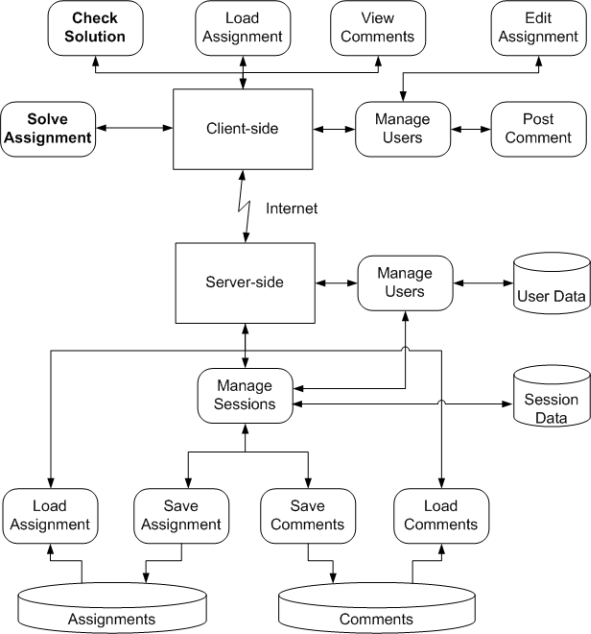
\includegraphics[width=0.85\textwidth]{./img/architecture01a.png}
		\caption{LDBN - System Architecture}
		\label{fig:sysarch}
	\end{center}
\end{figure}

It should be noted that the functions in the diagram represent many classes and 
static methods, which are all serving the same purpose/function. We are not 
going to discuss all 
of the functions in detail, because most of them are straightforward and 
self-explanatory. 

\subsubsection{Client-side Functions}

\begin{description}
	\item[Solve Assignment] function is used for generating a sample solution to 
		a given assignment, and presenting it to the user. As we mention in 
		Section~\ref{sec:introldbn}, an assignment consist of a relation schema in universal-relation form (URF).
	\item[Check Solution] function, as the name suggests, performs series of checks to 
		test the correctness of the given solution. A solution to an assignment consists 
		of a decomposition of the schema from URF into 2NF, 3NF and BCNF. In addition,
		the user must define one of the key candidates of each new relation in each
		decomposition. 
	\item[Load Assignment] function presents a list of all assignments, which are 
		stored in the database, to the user, and it can load new assignment from that list
		in the UI.
	\item[Manage Users] function allows unregistered users to create new account 
		and registered users to login with their password and username. 
	\item[Post Comment] function gives register users the ability to comment an assignment, 
		thus be able to communicate with all other users.
	\item[View Comments] function displays comments for each assignment, posted by registered users.
	\item[Edit Assignment] function provides registered users with the 
		ability to create, edit, save, export and import assignments. 
\end{description}

As we can see from Figure~\ref{fig:sysarch} the functions \textit{Post Comments} 
and \textit{Edit Assignments} do not directly communicate with the Server-side, but rather 
communication goes first trough the \textit{Manage Users} function. This is done in order 
to ensure that the users are properly logged in into the system before attempting 
to use those functions. We will refer to functions which require users to login as restricted. 

The functions \textit{Solve Assignment} and \textit{Check Solution} are definitely the most 
important functions of LDBN, therefore we are going to illustrate how they perform their tasks
in more detail in Section~\ref{sec:keyfunctions}. 

\subsubsection{Server-side Functions}

Most of the functions on the server-side are used as communication links (CL) for the
functions on the client-side to the database. This means, they retrieve/store data form/in the 
database, then convert the data to a XML string and send it back to the client-side
functions. 

\begin{description}
	\item[Load Assignment] is the CL for the \textit{Load Assignment} function on the 
		client-side.
	\item[Load Comments] is the CL for the \textit{View Comments} function.
	\item[Manage Sessions] function ensures that the data is coming from a registered user.
		is also responsible for creating a new session, and killing an existing one. Furthermore,
		each session has an unique ID, which is generated and send back to the user 
		when he/she has logged in. This ID is stored in the \textit{Session Data} and it is used for
		legitimizing the user in order for him/her to obtain access to restricted functions.
	\item[Manage Users] function is the CL of the \textit{Manage Users} on the client-side.
		It is responsible 
		for inserting new users into the database and for modifying existing data such as 
		username, password and email.
		It uses the \textit{Manage Sessions} function in order to ensure that an 
		user is always logged in, before he/she atemps to change any user data.  
	\item[Save Assignment] is CL for the \textit{Edit Assignment} function on the client side. 
		It is a restricted function, thus it uses the \textit{Manage Sessions} function. 
	\item[Save Comment] is CL for the \textit{Post Comment} function on the client-side, it is 
		a restricted function as well.
\end{description} 

\section{Core Package of LDBN}
Before moving to Section~\ref{sec:keyfunctions}, where we discuss the  most important functions of 
LDBN namely the \textit{Solve Assignment} and the \textit{Check Solution} functions, 
we are going to present the core package of LDBN. This package contains the foundation 
classes, on which both of the functions functions depend, therefore it is an essential 
part of LDBN. 

Before going into more detail, we are going to present the different data items in LDBN. 
We refer to data items as items nececary to describe a database schema.  
The three key items in the implementation are relations, FDs, and keys.
Figure~\ref{fig:relexample} is illustrating
an (abstract) example of those data items and their structure in our system. 
As can be seen, the most important data item is the relation, since
it holds the other two data items. This suggests itself, because FDs and keys have meaningful
interpretation only in combination with a relation. Furthermore, a key is a subset of 
the relation's attributes, and
each relation can have a set of FDs. On the other hand, 
each FD contains of two subsets of
the realation's attributes, these represent the left-hand side (LHS) and the 
right-hand side (RHS) of a FD. Finally, a database schema or a decomposition of
a database schema can be described as a set of relations.


\begin{figure}[h]
	\begin{center}
		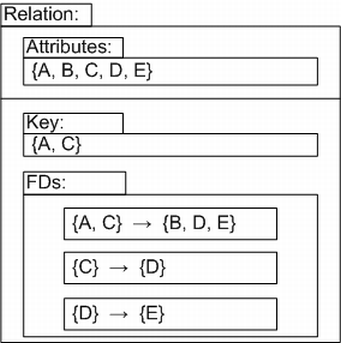
\includegraphics[scale=0.5]{./img/relation-example01a.png}
		\caption{Example of a Relation}
		\label{fig:relexample}
	\end{center}
\end{figure}

At this point the reader schould be familiar with the different data items 
and we can go into more detail of the 
actual implementation of the different data stcutures in LDBN which are holding 
the data items. Figure~\ref{fig:coreuml} shows an UML class diagram of the most important 
classes and methods of the package. 

\begin{figure}[h]
	\begin{center}
		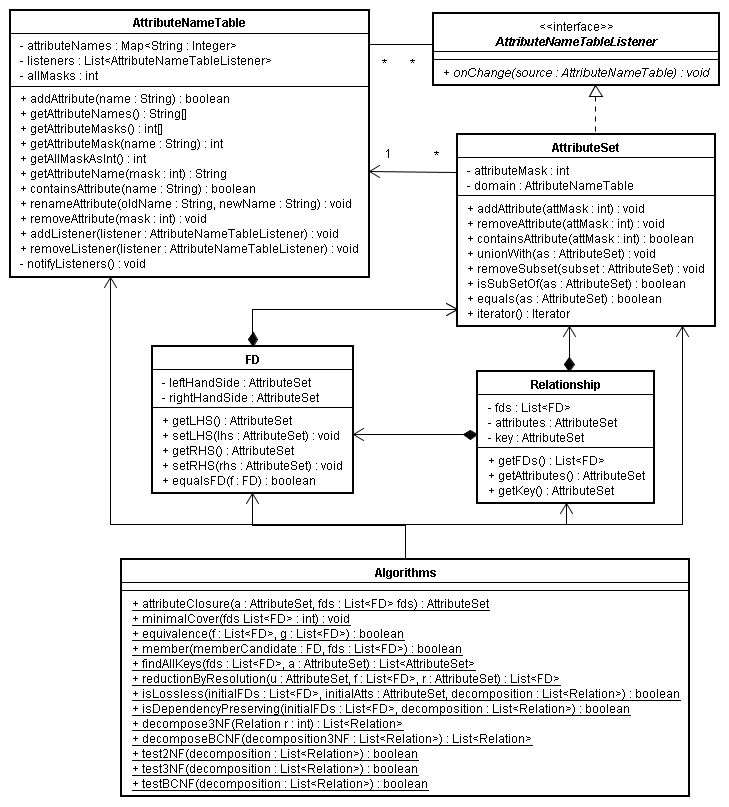
\includegraphics[width=0.9\textwidth]{./img/uml02.png}
		\caption{LDBN - Core Classes}
		\label{fig:coreuml}
	\end{center}
\end{figure}

As the reader may have noticed, each data item consists of attributes and/or other
data items, therefore the \verb=AttributeSet= class is a fundamental class in LDBN. 
It holds attributes of a relation. 
In the early stages of the implementation of LDBN attribute sets
were simply represented as arrays of strings. However, this has proven to be very
inefficient even for trivial operations like comparation or union of two sets. This could 
lead to efficiency problems with
bigger assignments, since set operations are used quite often due to the exponential
complexity of many algorithms in LDBN.
The solution was to use a variable of type integer as a representation of an entire
attribute set. 
This way attributes are added or removed from the set by using the bit operators, 
thus every attribute is 
a bit index in the integer variable. This has the disadvantage that
assignments can contain only up to 32 attributes, but exceeding 32 attribute 
is highly unlikely to happen in an educational software. On the other side, the 
advantages are of much greater value, as set operations, which are used quite 
often, are performed in almost constant time, since we are using bit operators only.
For example, if we want to make the union of two sets, we just use the 
bitwise OR operation on both integer variables.
 
Every \verb=AttributeSet= object has an associated domain name space called 
\verb=AttributeNameTable=. 
It contains a map, so that the string name of an attribute is mapped to its 
integer representation. In this way information is never lost. It is worth mentioning 
that initially a long variable was used
instead of an integer. This gave us 64 possible attributes in an assignment, 
however, JavaScript has only one numeric data type, which is the double. 
Double has only 53 bits of precision, thus if one want a "real" long integer with 64 bit, 
it has to be emulated. This could hurt the performance of an application~\cite{wgio1}, 
therefore we switched to integers in LDBN. Furthermore, the \verb=AttributeNameTable=
class uses the Event Listener design pattern, as a result of which classes implementing 
the \verb=AttributeNameTableListner= interface can update their content,
whenever changes in the \verb=AttributeNameTable= occur. This is used by instances of the 
\verb=AttributeSet= class, but also by some UI classes, which are not shown in the diagram. 

With the help of the \verb=AttributeSet= class we can easily implement the different data items.  
First, a key item is only an instance of the the \verb=AttributeSet= class. Second, there is the
\verb=FD= class, which is basically a composition of two \verb=AttributeSets=, 
each one representing the LHS and RHS of the FD. Finally, the \verb=Relationship= class 
holds a relationship, which consists of attributes, 
list of FDs and a key. 
\verb=Algorithm= class contains all of the algorithms described in Chapter~\ref{chap:preliminaries} as
static functions. Some of the algorithms have exponential complexity in the worst
case, therefore a lot of the produced output is being cached. This increases the
memory usage, but it could make the application respond much quicker, which
in our opinion is more important for the user.    

In the next section we are going to illustrate how LDBN uses the different algorithms
to perform the \textit{Solve Assignment} and the \textit{Check Solution} functions.

\section{Key Functions of LDBN}
\label{sec:keyfunctions}
As we stated earlier, the two most important functions of LDBN are the \textit{Solve Assignment} and 
the \textit{Check Solution} functions. They build the foundation of the system and
without them UI will loose its purpose, therefore we are going to
discuss the two function more formally in this section.

\subsubsection{Solve Assignment}  
The \textit{Solve Assignment} function can provide the user with a sample solution
to an assignment, thus it decomposes a database schema from URF into 3NF and BCNF. This
task involves many different algorithms. Figure~\ref{fig:orderdecomposition} is 
illustrating the order of how those algorithms are being applied.

\begin{figure}[h]
	\begin{center}
		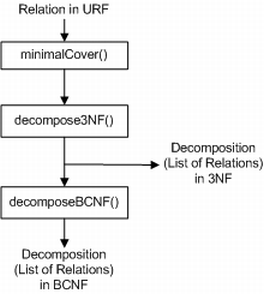
\includegraphics[scale=0.6]{./img/decomposition1a.png}
		\caption{Order of the Decomposition Algorithms}
		\label{fig:orderdecomposition}
	\end{center}
\end{figure}

First, the schema is passed trough the
\verb=minimalCover()= method of the \verb=Algorithms= class. There the all the
FDs of the schema are reduced in order to eliminate unnecessary FDs so that only 
a minimal number of dependencies remains. After that we use the \verb=decompose3NF()=
method, which implements the decomposition algorithm described in the textbook of 
Kemper and Eickler~\cite{bdb2}. The algorithm was presented in Section~\ref{sec:algdec}.
For quick reference, in this algorithm first we find all the key candidates of
the initial relation, this is necessary in order to determine later if one of them
is present in the new relations of the decomposition, which is required by the algorithm
to ensure dependency preservation. After that, we build new relations corresponding
to each FD, after they have been reduced. Then we need to eliminate relations, the attributes
of which are subset of the attributes of another relation. Finally we need to associate a
key for each of the new relations. The produced set of relations is dependency preserving and
it is in 3NF.

For computing the BCNF decomposition we use a slightly modified algorithm than the one described
in by Kemper and Eickler~\cite{bdb2}, which we described in Section~\ref{sec:algdec}. In our implementation
the input for the algorithm is not the initial schema in URF, but the decomposition
produced by the \verb=decompose3NF()= method. By doing this we 
increase the performance of the system, since many decompositions which 
are in 3NF are also in BCNF, or the differences are usually rather small, thus the algorithm
requires fewer passes.   

The reader may have noticed that LDBN does not provide an algorithm for decomposing a schema into
2NF. As we mention in Chapter~\ref{chap:preliminaries}, every decomposition
which is in 3NF is also in 2NF, and every
decomposition in BCNF is also in 3NF. Thus we could theoretically decompose the schema only 
into BCNF and present it as a solution for 2NF, 3NF and BCNF. However, a dependency 
preserving decomposition in BCNF is not always possible~\cite{bdb1, bdb2, bdb3, bdb3}. 
Because of this, we also present a dependency preserving 3NF decomposition, which is always
possible to find.   

\subsubsection{Check Solution}  
The \textit{Check Solution} function of LDBN allows the system to test a solution 
provided by the user and assess its correctness to many factors, which
we are going to present later in this section. As we mention in Chapter~\ref{chap:introduction} 
and~\ref{chap:preliminaries}, it is not possible
to compare a solution produces by LDBN with the one of the user, since they may be many
possible solutions/decompositions to a certain database schema. Therefore we need the
algorithms for testing a decomposition described in Section~\ref{sec:algtest}. In this section
we are going to illustrate how we apply those algorithms in our implementation. 

First of all, a solution in LDBN is represented as a list of instances of the
\verb=Relation= class. Those objects are build from the user input. The list is then
passed to the static functions in the \verb=Algorithm= class, which 
implement the all of the algorithms described in Section~\ref{sec:alg}. 
The system analyzes the solution to the following factors:

\begin{description}
	\item [Losses Join] properly for every decomposition. This check is done by directly applying the 
		algorithm \textit{Lossless Join Property Test}, which is 
		implemented by the \verb=isLossless()= method.
		
	\item [Dependency Preservation] for every decomposition. This check is done by directly applying the 
		algorithm \textit{Dependency Preservation Test}, which is implemented by the 
		\verb=isDependencyPreserving()= method.
		
	\item [Correctness of the FDs] of each relation, this means, testing if the FDs associated by the user
		for each new relation are actually in the closure of FDs for this relation. We do this by
		using the \textit{Reduction by Resolution} algorithm for computing the embedded closure of FDs for the given
		relation. This algorithm is implemented by the \verb=reductionByResolution()= method. Then we apply
		the \textit{Equivalence} algorithm to test if both set of FDs, the one produced by 
		the algorithm and the one provided by the user, are equivalent. Here the \textit{Reduction by Resolution}
		algorithm can have exponential complexity in some bad cases~\cite{p4}, therefore we cache the results
		of the algorithm for future use, e.g., when the user needs to recheck his solution, which can happen
		quite often during the process of solving an assignment correctly. 
		
		Here it should be noted that
		eventough the \textit{Dependency Preservation} factor ensures that every FD from the URF is preserved
		in the new decomposition, it does not give any information if the FDs provided by the user 
		for a certain relation are
		applicable on the subset of attributes for that relation. Therefore this factor is very important 
		in order to ensure the correctness of the following checks. 
		
	\item [Correctness of the Key] of each relation. This check is performed by first computing 
		every possible key candidate
		for each new relation, by applying the algorithm \textit{Finding All Key Candidates}, 
		which is implemented
		by the \verb=findAllKeys()= method. The method returns a list of all possible key candidates
		for a given relation. Then the system searches if the key suggested by the user is 
		present in that list. The algorithm is quite slow due to the fact that the problem of
		finding all key candidates is know to be NP-complete~\cite{p3}. To improve performance LDBN
		caches every list found for each relation, so that whenever a user needs to rechecks his/her solution
		the system computes only the lists of key candidates for new, uncached relations.  
		
	\item [Correctness of the Decomposition] in this check we apply directly the 
		\textit{2NF, 3NF, BCNF Properly Test} algorithms described in 
		Section~\ref{sec:algtest}. The algorithms are implemented by the 
		\verb=test2NF()=, \verb=test3NF()=, \verb=testBCNF()= methods.
		
\end{description}

All the checks are performed in the exact order described above. If one of the checks fails the following ones
are not executed. This way we are able to give the user a faster feedback, because 
the most computationally expensive checks are at the end. For example, if the \textit{Dependency preservation}
check, which is performed in polynomial time, fails, then the other check such as the 
\textit{Correctness of the Key} and the \textit{Correctness of the Decomposition}, both of which 
have exponential complexity, are omitted, thus the user could get a much faster response from the system
in case of an error. 

\section{User Interface}
The most important part of a system for end users and critical for system 
success is the UI~\cite{p9}, as such we put most of
our efforts in developing a fast, intuitive and stable UI. Furthermore,
it is possible to define two distinct user groups, warranting at least two different
user interfaces for LDBN.  One group would include the lecturers, who will
focus their attention on creating assignments. The other group would be the 
students, who will use the leaning environment mostly for solving 
the assignments provided by the lecturers. It should be noted, that every registered
user can create assignments, thus students can take the role of lecturers as well.
We tried to provide both 
user groups with fast and easy to use UI. In order to achieve this we put a lot
of our attention in finding a good layout for the UI. The requirements for
the layout were to give the user as much information possible about an 
assignment without loosing the general view. In order to achieve this goal  
we split the UI in four different views using tabs:

\begin{description}
	\item[Home] view is where the users can login, register and view some information 
	about the learning environment. It can be seen in Figure~\ref{fig:hv}.
	\item[Solve Assignment] view is where students can load an assignment, give and
	test their solutions. In case they have troubles finding the right solution
	LDBN could generate a sample one and present it. Figure~\ref{fig:sav} is showing
	the view with a loaded assignment.
	\item[Create Assignment] view is used by lecturers to create, edit, export or import
	assignments. It can be seen in Figure~\ref{fig:cav}.
	\item[License] view displays a license information about LDBN.
\end{description} 

\begin{figure}[h]
	\begin{center}
		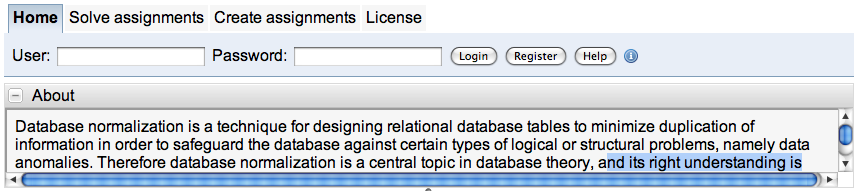
\includegraphics[width=0.85\textwidth]{./img/screen-tab1.png}
		\caption{Home View}
		\label{fig:hv}
	\end{center}
\end{figure}

\begin{figure}[h]
	\begin{center}
		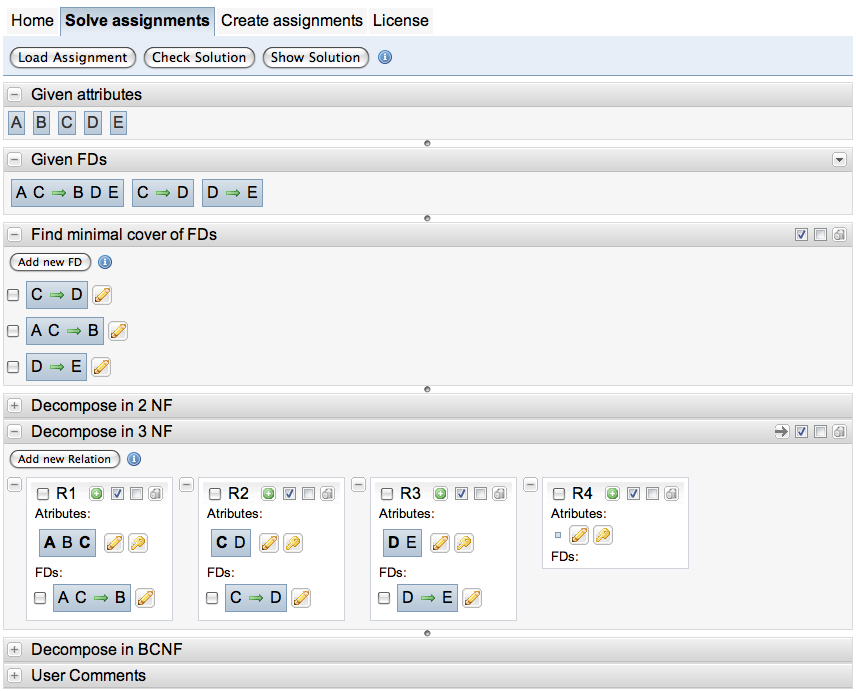
\includegraphics[width=0.85\textwidth]{./img/screen-tab2.png}
		\caption{Solve Assignments View}
		\label{fig:sav}
	\end{center}
\end{figure}

\begin{figure}[h]
	\begin{center}
		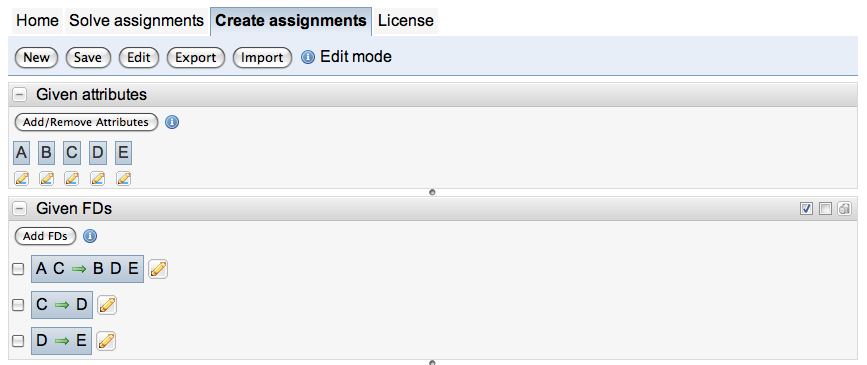
\includegraphics[width=0.85\textwidth]{./img/screen-tab3.png}
		\caption{Create Assignments View}
		\label{fig:cav}
	\end{center}
\end{figure}


\subsubsection{Solve Assignment View}
The most important view for students is definitely the \textit{Solve Assignment} view.
It contains the following fields:

\begin{itemize}
	\item Given attributes.
	\item Given FDs.
	\item Minimal Cover.
	\item 2NF, 3NF, BCNF Decomposition.
	\item Comments.
\end{itemize}

The \textit{Given Attitibutes} and the \textit{Given FDs} fields are not editable
and they correspond	to the information stored in each assignment, which is all the 
attributes and all the FDs of a database schema in URF. In all other fields 
the content can be modified by the user using different editors,
such as the \textit{Attribute Editor} (Figure~\ref{fig:attedit}), 
the \textit{Key Editor} (Figure~\ref{fig:keyedit}) and the \textit{FD Editor}
(Figure~\ref{fig:fdedit}).
All of those editors contain one or two text boxes, where users can input 
different attribute names separated by commas
in order to define respectively attributes of a relation, a key or a set of FDs. With
the help of the editors the user can define relations like the one shown on 
Figure~\ref{fig:relui}. In this example we have a relation with attributes 
\textit{\{A, B, C\}}, a key \textit{\{A, C\}} and only one FD in the set of FDs,
namely \textit{\{A, B $\rightarrow$ C\}}.  Furthermore,
each of the editors is wrapped in a draggable dialog window. 
This way the editors do not require any space on any of the fields, 
and can be open only when they are needed. In addition to this, every attribute and every FD,
like the ones shown in the relation on Figure~\ref{fig:relui}, can be dragged and
dropped in the text box of each editor, as a result of which the attributes/FDs
are automatically inserted in the text areas of the editor.
This can help user define attributes, keys or
FDs much quicker, which on the other hand can help improve the usability of 
the learning environment. 

\begin{figure}[h]
	\centering
	\subfigure[Attribute Editor]{
		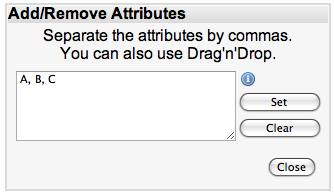
\includegraphics[scale=0.4]{./img/screen-atteditor.png}
		\label{fig:attedit}
	}
	\subfigure[Key Editor]{
		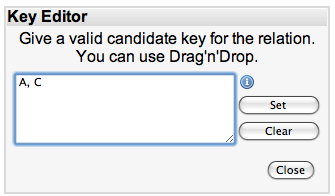
\includegraphics[scale=0.4]{./img/screen-keyeditor.png}
		\label{fig:keyedit}
	}
\caption{Attribute and Key Editor}
\end{figure}

\begin{figure}[h]
	\centering
	\subfigure[FD Editor]{
		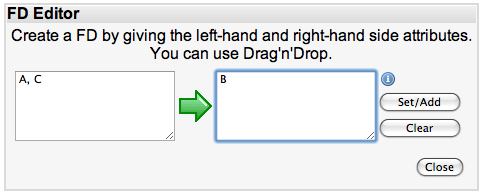
\includegraphics[scale=0.4]{./img/screen-fdeditor.png}
		\label{fig:fdedit}
	}
	\subfigure[Relation]{
		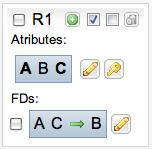
\includegraphics[scale=0.52]{./img/screen-rel.png}
		\label{fig:relui}
	}
\caption{FD Editor and an Example of a Relation in LDBN}
\end{figure}

We continue with the different fields in \textit{Solve Assignment} view. 
The first one is the \textit{Minimal Cover} field, where the user has to define 
a set of FDs using the \textit{FD Editor}. The user defined FDs must
build a minimal (canonical) cover of the \textit{Given FDs}.
This field is intended to be an intermediate step, which will help the user 
find easier a right decomposition
in the \textit{2NF, 3NF and BCNF Decomposition} fields. Those last three fields all
work the same way, with the only difference that the alogotithms for checking the 
correnctnes of the 
decomposition are are not the same.  
In each decomposition field the user must define a set of relations, like the one shown 
in Figure~\ref{fig:relui}. All the relations
within a filed represent a decomposition. To check the decomposition the user must
use the \textit{Check Solution} button, 
after that the system analyzes the solution by the criteria described in 
Section~\ref{sec:keyfunctions} and show a dialog with the result 
like the one in Figure~\ref{fig:screen03} 

Another useful feature, which also improves the usability of LDBN and greatly reduces
the time for defining relations, 
is the ability to 
import entire decompositions from the 2NF into the 3NF field, and from the 
3NF field into the BCNF field. This was done, because usually 
the differences between the decompositions are not huge, and each decomposition
can be used as a good staring point for the other ones.	

The last field of the \textit{Solve Assignemtn} view is the \textit{Comment} field, 
where users can view and post textual comments on every assignment.

\subsubsection{Create Assignment View}
The \textit{Create Assignment} view looks very similar to the 
\textit{Solve Assignment} view. It also has a \textit{Given Attributes} and 
\textit{Given FDs} fields. However, in this view these fields
can be edited using the \textit{Attribute Editor} and the \textit{FD Editor}. 
This allows users to define new assignments or modify existing ones. In addition, the view
allows users to save the assignments in the database or to export them as XML
files to the local file system. Importing an assignment form a XML file is also 
possible.  
\newline
Finally, in case the user needs any help with certain aspects of LDBN, the system provides 
help dialogs for every key feature of the UI. The dialogs can be open
using information buttons (
\includegraphics[scale=0.5]{./img/info.png}), which can be
found near every button or in every editor. This way help information is 
visually organized and the user has fast access to it. An example of such help dialog
window is shown in Figure~\ref{fig:screen-help}.

\begin{figure}[h]
	\begin{center}
		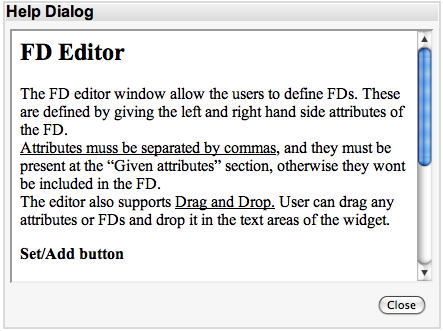
\includegraphics[width=0.5\textwidth]{./img/screen-help.png}
		\caption{Help Dialog for the FD Editor}
		\label{fig:screen-help}
	\end{center}
\end{figure}


\section{Server-side}
The server-side is mainly used for persistent storage of assignments, user comments,
user and session data. The communication between the web server and the client
is done using the POST method of the Hypertext Transfer Protocol - HTTP/1.1~\cite{w6}.
The POST method has two advantages over the GET method. First, it is more secure, i.e., 
the GET method is defined as safe, which means it is intended only for information 
retrieval and should not change the state of the server. Second, although the
RFC 2616, "Hypertext Transfer Protocol -- HTTP/1.1"~\cite{w6} does not specify
any requirement for URL length, many browsers like Internet Explorer limit
the length of an URL to a maximum of 2048 characters. This length may not be 
enough for LDBN, as it sometimes sends very large assignments back to the server.  

The web server uses XML to send data back to the client. LDBN defines its own XML data
exchange format. The format has several types:

\begin{description}
	\item[Message] for sending string messages, which appear in an alert window on 
	the client-side. Such messages can be for instance an error messages returned
	by the database. 
	\item[Comments] for sending user comments. 
	\item[Session] contains session data for logged in users such as an unique session 
	ID, generated by the server and stored in the database. The ID is used for
	legitimizing user actions on the server-side.
	\item[Assignment List] for sending back meta data for each assignment. This
	information is used by the \textit{Load Assignment} function in order 
	to display a list of all available assignments from the database.
	\item[Assignment] contains a LDBN assignment. 
\end{description}  

\section{Security Issues}
The system uses HTTP 1.1 for the communication between the client and the web
server. This can easily be secured by using HTTPS instead. The upgrade only
require changes to the configuration of the web server. However, using an encrypted
connection does not prevent web applications from SQL injection and cross-site 
scripting attacks. SQL Injection refers to the technique of 
inserting SQL statements into web-based input fields in 
order to manipulate the execution of the SQL queries. Cross Site Scripting 
attacks work by embedding script tags into the web pages. 

Here follows a short example of a SQL injection.
Assuming that we have a poorly implemented PHP script for loading an assignment,
which has the following line of code in it:

\begin{verbatim}
     $sql_statement := "SELECT * FROM assignment WHERE id=$_GET['id'] ";
\end{verbatim}

\noindent If the "id" argument of the GET method is crafted in a specific way by a 
malicious user, the SQL statement may do more than the code author intended. 
For example, setting the "id" argument as:

\begin{verbatim}
     1; DROP TABLE users;
\end{verbatim}

\noindent yields the following SQL statement:

\begin{verbatim}
     SELECT * FROM assignment WHERE id=1; DROP TABLE users;
\end{verbatim}

\noindent The statement would cause the deletion of the "users" table. 

In order to prevent SQL injection and cross-site 
scripting attacks LDBN uses regular expressions for validating
user input, and it escapes HTML special characters like \lt and~\gt.
To the best of our knowledge, it is not possible to perform such attacks on LDBN.

Another issue with web-based applications is password protection. LDBN uses the 
MD5~\cite{w7} one-way encryption algorithm for hashing user passwords. 
To authenticate an user, the password presented by him/her is hashed on the client-side, 
then send to the web server and compared with the stored hash in the database. 
This way the actual password of the user is never sent over the network.
